\documentclass[a4paper,10pt]{article}
\usepackage[utf8]{inputenc}

\usepackage[english]{babel}
\usepackage[dvinames]{xcolor}
\usepackage[compact,small]{titlesec}
\usepackage{booktabs}
\usepackage{multirow}
\usepackage{amsfonts,amsmath,amssymb}
\usepackage{marginnote}
\usepackage[top=1.8cm, bottom=1.8cm, outer=1.8cm, inner=1.8cm, heightrounded, marginparwidth=2.5cm, marginparsep=0.5cm]{geometry}
\usepackage{enumitem}
\setlist{noitemsep,parsep=2pt}
\newcommand{\highlight}[1]{\textcolor{kuleuven}{#1}}
\usepackage{pythonhighlight}
\usepackage{cleveref}
\usepackage{graphicx}
\usepackage{algorithmic}

\newcommand{\nextyear}{\advance\year by 1 \the\year\advance\year by -1}
\newcommand{\thisyear}{\the\year}
\newcommand{\deadlineGroup}{November 27, \thisyear{} at 16:00 CET}
\newcommand{\deadlineCode}{December 18, \thisyear{} at 16:00 CET}
\newcommand{\deadlineReport}{January 4, \nextyear{} at 16:00 CET}

\newcommand{\ReplaceMe}[1]{{\color{blue}#1}}
\newcommand{\RemoveMe}[1]{{\color{purple}#1}}

\setlength{\parskip}{5pt}

%opening
\title{Evolutionary Algorithms: Final report}
\author{Stijn Staring (r0620003)}

\begin{document}
\fontfamily{ppl}
\selectfont{}

\maketitle

%\section{\RemoveMe{Formal requirements}} \label{sec_this}

\section{Metadata}

\begin{itemize}
 \item \textbf{Group members during group phase:} Rajat Sharma and
 Pieter-Jan Vrielynck \\
 \item \textbf{Time spent on group phase:} 13 hours
 \item \textbf{Time spent on final code:} 82 hours
 \item \textbf{Time spent on final report:} 12 hours\\
\end{itemize}

\section{Modifications since the group phase}

\subsection{Main improvements} 

\paragraph{1 Inver-over operator:}\label{p:1}The final implementation of the evolutionary algorithm makes use of an inver-over operator \cite{inver_over}. This operator tries to combine the advantage of unary operators (mutation) and binary operators (cross over), which have respectively low calculation cost and a notion of the population. During both mutation and cross over an inversion takes place of a subset of the selected route. While the first inversion point is determined as explained in  Section \ref{s:cross_over}, the second one is randomly selected during mutation and population driven during cross over. The process of consecutive variations on the selected route, goes on for a non-fixed amount of time.\\
 The inver-over operator replaces the sequential constructive cross over and the scramble mutation operators used during the group phase. ``SCX'' is a suitable operator but not efficient enough for big problems and scramble is a naive method that breaks a lot of edges and can therefore damage good solutions.  

\paragraph{2 Enrichment of the initial population:}\label{p:2} The ``Nearest Neighbours'' heuristic is used to initialize the population. In order to enhance the diversity it is not allowed to start multiple times from the same city when building up a solution. Afterwards the local search technique ``3-opt'' is applied for a couple of iterations. This local search technique is also used after the variation operators. After initialization of the population a best solution of $28074$ is attained in $0.69$ seconds for the tour29 problem which is better than the mean best solution during the group phase which was around $32250$. For this result population size was set to $100$ and the amount of iterations of the ``3-opt' local search operator to $ 1 $.

\paragraph{3 Parallel selection and elimination:}\label{p:3} After retrieving a good initial population, each individual is sequentially chosen to be adjusted by means of variation operators. After a variable amount of adaptations the offspring is compared with its parent and the most fittest solution is included in the next generation. 

\paragraph{4 Applying the ``3-opt'' local search operator on the offspring:} When the offspring is created, the ``3-opt'' local search operator is applied for a couple of iterations. ``3-opt'' can be summarized as looking for the replacement of three edges which will lead to a better objective value.
However, the domain of possible combinations of edges to remove is too big to test directly so a notion of which edges have the most potential to lead to an improvement should be present. Therefore, each time before three edges are removed two local searches are performed to identify the most promising ones.

\subsection{Issues resolved}

\paragraph{Slow algorithm due to high calculation load:} When applying the algorithm of the group phase to the bigger problems e.g. tour $194$, the algorithm became very slow. Solutions attained were therefore of poor quality. The calculation load is still high due to the vast size of the TSP's, but it is mitigated by the use of the cheap inver-over operator (see Section \ref{p:1}).  Also, the optimal population size is chosen to make an optimal trade off between  calculation load and quality of the solution.

\paragraph{Worse results than simple greedy heuristic:}Because of the use of a rich initial population (Section \ref{p:2}) the genetic algorithm already starts from a solution better than the simple greedy heuristic. This means that the gap that it has to bridge to reach the optimal solution is made much smaller.

\paragraph{Instantaneous loss of diversity:} During the group phase good solutions rapidly took over the population which caused the algorithm to get stuck early in a local minima. This could be seen because the mean cost and the best cost quickly converged to each other which indicates that the diversity was completely gone. Therefore, the algorithm was not able to reach the optimal solution. The mean value of the best solution was still around a cost of $4000$ away from the optimal solution after $10$ complete runs of the smallest problem. Additionally, there was a lot of variation on the solutions. This follows from the poor domain exploration, whereby the local minima that were reached are mainly based on random factors during the initialization of the population, the selection operator and the mutation operator. The reason for a rapid loss of diversity was a too high exploitation pressure that was introduced by making use of the $\lambda/\mu$ - elimination scheme in combination with a too high k value during k-tournament selection. Also, the population was initialized by introducing random routes. This not necessarily lead to a diverse population. \\ Because the inver-over operator only copies one edge at a time during cross over with a different individual and because a variable amount of cross overs with random individuals and mutations take place after which the ``3-opt'' local search is applied, the population is not easily taken over by good individuals and the population remains diverse.

%With the implementation of a parallel selection and elimination operator good solutions taking over the population is avoided. 

\paragraph{Increasing cost of the best solution:} During testing in the group phase it was found that the best solution sometimes increased in cost. Because a $\lambda/\mu$ - elimination scheme was used the reason for this will have been the mutation operator. By making use of the parent vs offspring comparison in the current implementation this behaviour is avoided. 


\section{Final design of the evolutionary algorithm:} 
%\RemoveMe{\textbf{Goal:} Based on this section, we will evaluate insofar as you are able to design and implement an advanced, effective evolutionary algorithm for solving a model problem.}
%
%\ReplaceMe{In this section, you should describe all components of your final evolutionary algorithm and how they fit together.}

\subsection{Representation}

Each individual solution is represented by an object of the Travelling Sales Man class. This structure allows for grouping different features i.e. cost of the route and the route followed itself. The order of the cities visited matches with the order of numbers that are listed and wherefore each number identifies a city.  Lists are easy to modify and a lot of build in operators can be used. Also the list can intuitive be converted to a graph notation by assigning an edge from the current city to the city on the next index. During cost calculation, the cost of the edge between the last and the first element should not be forgotten.

\subsection{Initialization}

The population is initialized in two steps. The first step comprises a ``Nearest Neighbours'' heuristic and the second step applies a ``3-opt'' local search operator(see Section \ref{s:local_search}). \\The NN heuristic is implemented by choosing a random start city and always keep travelling from the current city to the nearest, next city. This automatically comes with the advantage of avoiding infinity costs and thus constructing a feasible solution even when not all the cities are interconnected. Additionally, to get a higher amount of diversity at a low calculation cost, it is expected to use every city only once to start from. It can be that the demanded population size is bigger than the amount of available start cities. In this case, after all the start cities have been used by the NN heuristic, randomly generated routes are inputted to the ``3-opt'' local search operator. The amount of iterations applied by ``3-opt'' is a parameter that is identified during the hyperparameter optimization. After initialization the best solution lays already close, in a range of $5\%$, from the optimal solution. The genetic algorithm is charged with the task to execute the final improvement.\\

For bigger problems a rather small population is chosen to cut the calculation load. For the tour $929$ for example, the initial population size is set to $ 10 $. As discussed earlier, because the inver-over operator only copies one edge at a time during cross over with a different individual and because a variable amount of cross overs with random individuals and mutations take place after which the ``3-opt'' local search is applied, the population is not easily taken over by good individuals and the population remains diverse.


\subsection{Selection operators}

During the development of the evolutionary algorithm, their was a constant push towards more simple and efficient methods because of the big size of the travelling salesman problems. The things that have been tried are listed as follows:

\begin{itemize}
	\item k-tournament with variable k-value
	\item Exponentially decreasing probability distribution function based on ranking
	\item Selecting every individual in the population 
\end{itemize}

K-tournament makes use of a competition based selection mechanism. The k-tournament operator was tried because the k value makes it easy to trade off exploration and exploitation and the operator can be easy and cheaply implemented. Next, it also introduces still some randomness. The optimal k-value can be identified during hyperparameter optimization. There has been experimented by stepwise increasing the k-value with the amount of generations. Choosing k equal to $1$ at the start of the algorithm, a random selection will apply and the focus is on exploration of the solution domain. By increasing the k-value over time, a shift towards exploitation of good solutions will take place. The use of the exponentially decreasing probability distribution function based on ranking gave similar results when using a decreasing s-value.\\

In the final implementation all individuals are consecutively selected to undergo a variable amount of variations. During cross over the second inversion point is identified by a different individual in the population. This different individual is randomly chosen from the population. The advantage to make use of this selection scheme is because it is cheap and no parameters should be identified. It could also be argued that using a competitive based selection mechanism in combination with a small population for the bigger problems i.e. a population size of $10$ during the tour 929 problem, will lead to a too big emphasis on possibly only slightly better individuals because of the high chance of being selected. 


\subsection{Mutation operators}\label{s:mutation}

A mutation operator functions as a random local search and introduces randomly new edges in the population. It is often applied with a small probability in order not to damage good solutions too hard. Mutation is an unary operator which means that it only takes one individual as input and the operator is not population driven.\\
The mutation that is chosen is a simple inversion of a subset of the individual. This could efficiently be implemented. The downside however for using such an operator is that it is not taking the asymmetry of the cost matrix into account. In effect it is thus changing more than two edges during inversion which can even lead to an infeasible solution when not all the cities are interconnected. By using this implementation it is thus assumed that the cost matrix behaves approximately symmetric. Therefore the ``Greedy Mutation''\footnote{Access to the other developed operators can be given through mail.} operator was developed as explained in \cite{Reisleben1996} but this didn't make it to the final design due to a too high calculation load when implemented. The ``Greedy mutation'' works by randomly choosing to remove between $4$ and $7$ edges from a candidate solution and in a greedy way reconnect all the different parts. This operator can deal with the asymmetry of the cost matrix in a better way.\\
The mutation rate is already chosen as a small number from the start, thus decreasing the probability of mutation over the generations is not necessary. Self-adaptivity can be used to determine the mutation rate of each individual. This however gave similar results as in the hyperparameter optimization.

\subsection{Recombination operators}\label{s:cross_over}

The recombination operator executes an inversion of a subset in a selected individual p1 where the second inversion point is based on a different individual p2 present in the population. The offspring o1 is initialized as the copy of p1. When it's turn to o1 to be adjusted, the variation starts by selecting randomly a city $c$. The edge after this city will be the first inversion point. A second city c' is chosen randomly in the case of mutation or the city after c in a randomly chosen other individual p2. The second inversion point is the edge after the city c'. Now that the two inversion points are identified, the subset between city c and city c' is inversed. After cross over the edge between city c and city c' that was first present in p2, is now introduced in o1. Consecutive mutations and cross over take place for a non fixed amount of time, whereafter o1 is compared with p1 during the elimination as explained in Section \ref{s:elimination}. As discussed in Section \ref{s:mutation} the inversion operator is not the ideal choice when dealing with the asymmetric TSP due to its unpredictability. the reason that it still made it to the final design is due to its low calculation load and the assumption that the cost matrix still behaves relative symmetric. Also here an alternative ``Greedy cross over''\footnote{Access to the other developed operators can be given through mail.} is tried but was discarded due to its calculation load.\\

Recombination is generally a binary operator with as goal to identify the good characteristics of the candidate solutions and transfer this to the offspring. For the TSP it is therefore important to look at the overlap of two solutions and copy this to the offspring. The ``Greedy cross over'' as introduced in \cite{Reisleben1996}, can be summarized as gradually building the offspring in a ``Nearest Neighbour'' way, while imposing that the edges that were common in both parents are present in the offspring. Gradually building up offspring is however much more expensive than inversing a subset of a route. The reason to pick inferior but cheap variation mechanism is balanced by a more expensive ``3-opt'' local search operator that is applied after obtaining the offspring. This local search operator is suitable for the ATSP as is discussed in Section \ref{s:local_search}. 


\subsection{Elimination operators}\label{s:elimination}

After the creation of the offspring and applying a local search technique in the elimination step, the offspring is compared with its original parent and the parent is only replaced in the population if it leads to an improvement. This is an age based elimination. The best candidate will always stay present in the population and up and down behaviour of the best solution is thus avoided.\\

An alternative implementation was tried that made use of a k-tournament elimination scheme with the additional condition that once a candidate was copied to the survivors, it is removed from the population and it is checked that the same routes were not included anymore to the survivors. This means that different solutions became more likely to be selected next. The k-tournament was an improvement in comparison with the $(\lambda + \mu)$-elimination scheme implemented during the group phase because it contains still a certain degree of randomness which leads to a lower exploitation pressure and thus more exploration.\\
A better approach that is looked into checks the amount of similar edges between different solutions and based on this decreases the fitness of an individual. This means that also the probability that an individual will be selected if it is already included in the survivors, is decreased. This implementation was however to calculation expensive. 

\subsection{Local search operators}\label{s:local_search}

The reason that ``3-opt'' and not ``2-opt'' for example is chosen, is because ``2-opt'' only looks at a subpath that can be inverted which may in the case of the ATSP alter the tour length unpredictably \cite{Reisleben1996}. ``3-opt'' instead looks at a subtour that can be inserted between two cities and which is possibly inversed. First the naive ``3-opt'' was implemented by swapping three randomly chosen edges and then looking at eight ways to reconnect them. If there was an improvement the swap was executed. However, a lot of checks needed to be done before improvement was found.\\ 
The later more efficient ``3-opt'' implementation is based on two local searches that identifies the most potential edges to be replaced as explained in  \cite{fast_alg}.\\
It is possible to let the local search run until ``3-opt'' optimality is reached, but this was only feasible for the smallest problem. 
%The reason to pick inferior but cheap variation mechanism is balanced by a more expensive but better local search operator as is discussed in Section \ref{s:local_search}. 


\subsection{Diversity promotion mechanisms}

%\ReplaceMe{Did you implement a diversity promotion scheme? If yes, which one? If no, why not? Describe the mechanism you implemented. In what sense does the mechanism improve the performance of your evolutionary algorithm? Are there parameters that need to be determined? Did you use an advanced scheme to determine them?}

In the current implementation diversity is ensured during the initialization of the population by always starting from a different start city as is discussed in section \ref{s:initiation_population}.
Because the inver-over operator only copies one edge at a time during cross over with a different individual and because a variable amount of cross overs with random individuals and mutations take place after which the ``3-opt'' local search is applied, the population is not easily taken over by good individuals and the population remains diverse.\\

There has also been experimented with a k-tournament that conditions on a diverse population after elimination as was discussed in Section \ref{s:elimination}. It is the most effective to impose diversity during the elimination step because this has a direct effect while imposing diversity during the selection step on the contrary, has only an indirect effect. 

%Say that added diversity promotion in the elimination, because than you have a direct effect. This is not the case when you add a diversity mechanism in the selection step, because cross over and mutation can influence the diversity of the population. 

\subsection{Stopping criterion}

Because measures are taken to promote the diversity of the population, the stopping criteria used during the group phase, that takes the difference between the mean of the mean objective values and the mean of the best objective values, is not suitable anymore. The stopping criteria used is adjusted to a maximum number of iterations that the best objective value stays constant. 
 \newpage

\subsection{The main loop}
%In the final version applied a for loop over the population. While an individual is selected a variable amount of cross overs and mutations are applied. 
%
%Because of the for loop to select the individuals and as will further explained in Section \ref{s:elimination}, there is only competition between a parent with its offspring. 

\textbf{List of used operators during the inver-over method:}
\begin{itemize}
	\item Nearest Neighbours
	\item 3-opt local search
	\item inver-over operator
	
\end{itemize}

\textbf{The algorithm of the inver-over method:}

\begin{algorithmic}
	\STATE Initialization of the population P using Nearest Neighbours
	\STATE Apply 3-opt local search
	\WHILE {Termination condition is not fulfilled} 
		\FOR{each individual $ S_{i} $ in P}
			\STATE $ S^{'} = S_{i} $
			\STATE select randomly a start city c from $ S^{'} $
			\WHILE{True}
				\IF{(random.rand() $\leq$ mutation rate)}
				\STATE Select the city $ c^{'} $ from the remaining cities in $ S^{'} $
				\ELSE
				\STATE select (randomly) an individual from P
				\STATE assign to $ c^{'} $ the next city to the city c in the selected individual
				\ENDIF
				\IF{the next city or the previous city of city c in $ S^{'} $ is $ c^{'} $}
				\STATE Apply 3-opt local search
				\STATE \textbf{exit} from the while loop
				\ENDIF 
				\STATE inverse the section from the next city of city c to the city $ c^{'} $ in $ S^{'} $ 
				\STATE $c = c^{'}$				
			\ENDWHILE
			\IF{(eval($S^{'}) \leq eval( S_i$))}
			\STATE $S_i =  S^{'}$
			\ENDIF
		\ENDFOR
	\ENDWHILE
\end{algorithmic}
\vspace{0.25cm}

During the report there is often an alternative ``Greedy Method'' method mentioned. The operators of the fully developed, but later discarded, method are listed below: 

\begin{itemize}
	\item Nearest Neighbour heuristic
	\item 3-opt local search operator after initialization and cross over
	\item k-tournament with changing k value over time
	\item Greedy Mutation
	\item Greedy Cross over
	\item k-tournament elimination with additional diversity condition
\end{itemize} 

This method was tested on the tour $ 194 $ problem with hand picked parameters. Solutions obtained where of the order $ 9700 $.

\subsection{Parameter selection}

%\ReplaceMe{For all of the parameters that are not automatically determined by adaptivity or self-adaptivity (as you have described above), describe how you determined them. Did you perform a hyperparameter search? How did you do this? How did you determine these parameters would be valid both for small and large problem instances?}
A hyperparameter optimization is run for following variables:
\begin{itemize}
	\item Population size: $ \lambda = [20,75,100,150] $
	\item Mutation rate: $ \alpha = [0.02, 0.15,0.25]$
	\item Amount of iterations of the ``3-opt'' local search: $ N = [1,3,5] $
\end{itemize}

The final parameters obtained are summarized in Table \ref{t:parameters} together with the best objective value, mean best objective value and the mean time. A hyperparameter optimization for the tour 29 problem is not necessary because it already consistently reaches optimal solutions with hand picked parameters. The hyperparameter optimization is performed by making the logical cores calculate in parallel. Each combination of parameters is solved $ 8 $ times and the best objective value, mean best objective value and mean time are the criteria used to compare different parameter combinations.

\begin{table}[h]
	\centering
	\begin{tabular}{|p{5.5cm}|p{2cm}|}
		\hline
		\textbf{Parameters} & \textbf{Value}\\ \hline
		Dataset  & tour194.csv\\ \hline
		Initial Population size $[-]$ & 75\\ \hline
		Probability for mutation $[-]$ & 0.02\\ \hline
		Iterations of 3-opt $ [-] $ & 3 \\ \hline
 		Termination value $[-]$ & 100\\ \hline
 		Best fitness obtained over $ 8 $ iterations $[-]$ & 9569.90\\ \hline
 		Mean best fitness obtained over $ 8 $ iterations $[-]$ & 9703.05\\ \hline
 		Mean calculation time over $ 8 $ iterations  $[s]$ & 300\\ \hline
	\end{tabular}
	\caption{Used parameters for the results shown for tour 100 and tour 194.}
	\label{t:parameters}
\end{table}


\section{Numerical experiments}

\subsection{Metadata}

%\ReplaceMe{What parameters are there to choose in your evolutionary algorithm? Which fixed parameter values did you use for all experiments below? If some parameters are determined based on information from the problem instance (e.g., number of cities), also report their specific values for the problems below.
%
%Report the main characteristics of the computer system on which you ran your evolutionary algorithm. Include the processor or CPU (including the number of cores and clock speed), the amount of main memory, and the version of Python 3.}

%\textbf{Parameters to choose from for the inver-over method:}
%\begin{itemize}
%	\item Population size: $ \lambda $
%	\item Mutation rate: $ \alpha $
%	\item Amount of iterations of loop of the ``3-opt'' local search: $ N $
%\end{itemize}

\textbf{Computer specs:}
\begin{itemize}
	\item Processor: Intel Core i7-5500U
	\item Physical cores: $ 2 $
	\item Logical cores: $ 4 $
	\item Clock speed: $ 2.40GHz $
	\item RAM: $ 12 GB $
	\item Python Version: $ 3.8 $
\end{itemize}


\subsection{tour29.csv}

The best tour length that is found is always the same and has a cost of $ 27154.49 $.
The tour that is associated with this cost is: \\
\begin{equation*}
Tour 29  = 	[21, 20, 16, 17, 18, 14, 11, 10, 9, 5, 0, 1, 4, 7, 3, 2, 6, 8, 12, 13, 15, 23, 24, 26, 19, 25, 27, 28, 22]
\end{equation*}

The parameters used to obtain the convergence plot were picked by hand and are listed here in Table \ref{t:parameters}. For the histograms the termination value is set on $ 50 $ instead of $ 20 $, to remove small variations in the objective values found.
\begin{itemize}
	\item Population size: $ 100 $
	\item Mutation rate: $ 0.02 $
	\item Amount of loops of the ``3-opt'' local search: $ 5 $
	\item Termination value: amount of times no different best solution: $ 20 $ 
\end{itemize}
  
Because the mean and best solution don't directly convergence to each other, it can be concluded that the problem of instantaneous loss of the diversity is solved. Also, the solution isn't changing much anymore after $ 15 $ seconds. The algorithm convergences consistent to the optimal value. 


\begin{figure}[h]
	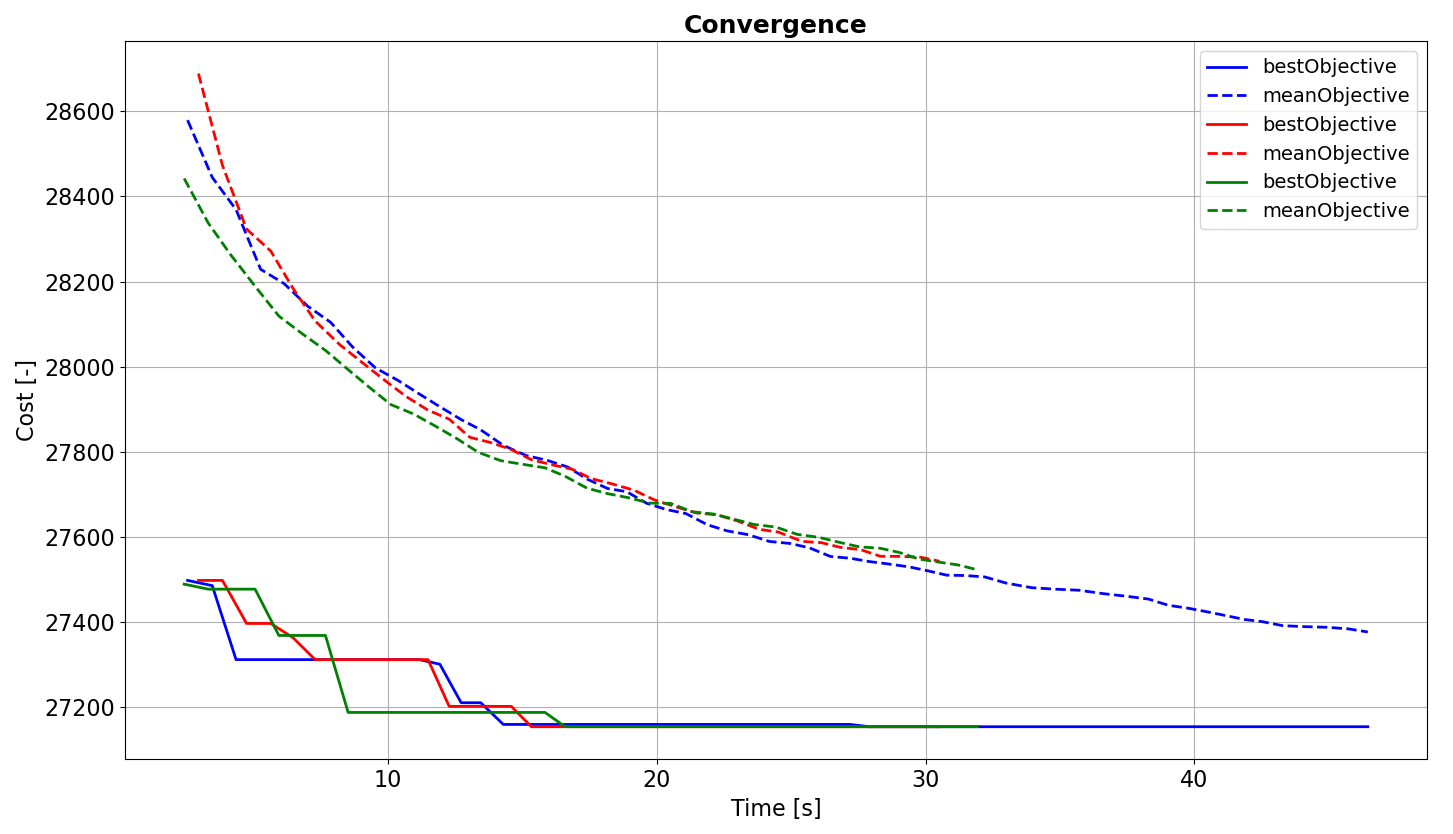
\includegraphics[width=1\textwidth]{Convergence_tour29.PNG}
	\caption{Convergence plot of the tour 29 TSP}
	\label{fig:convergence_tour29}
	\centering
\end{figure}

The mean best solution and the standard deviation of the tour 29 TSP after $ 1000 $ runs is given by ...  and ... respectively. Figure\ref{label} and \ref{ } show the distribution of the best and the mean solution. It can be concluded that optimal solutions were consistently found for the tour29 problem.  

%\begin{figure}[h]
%	\label{fig:hist_best_sol}
%	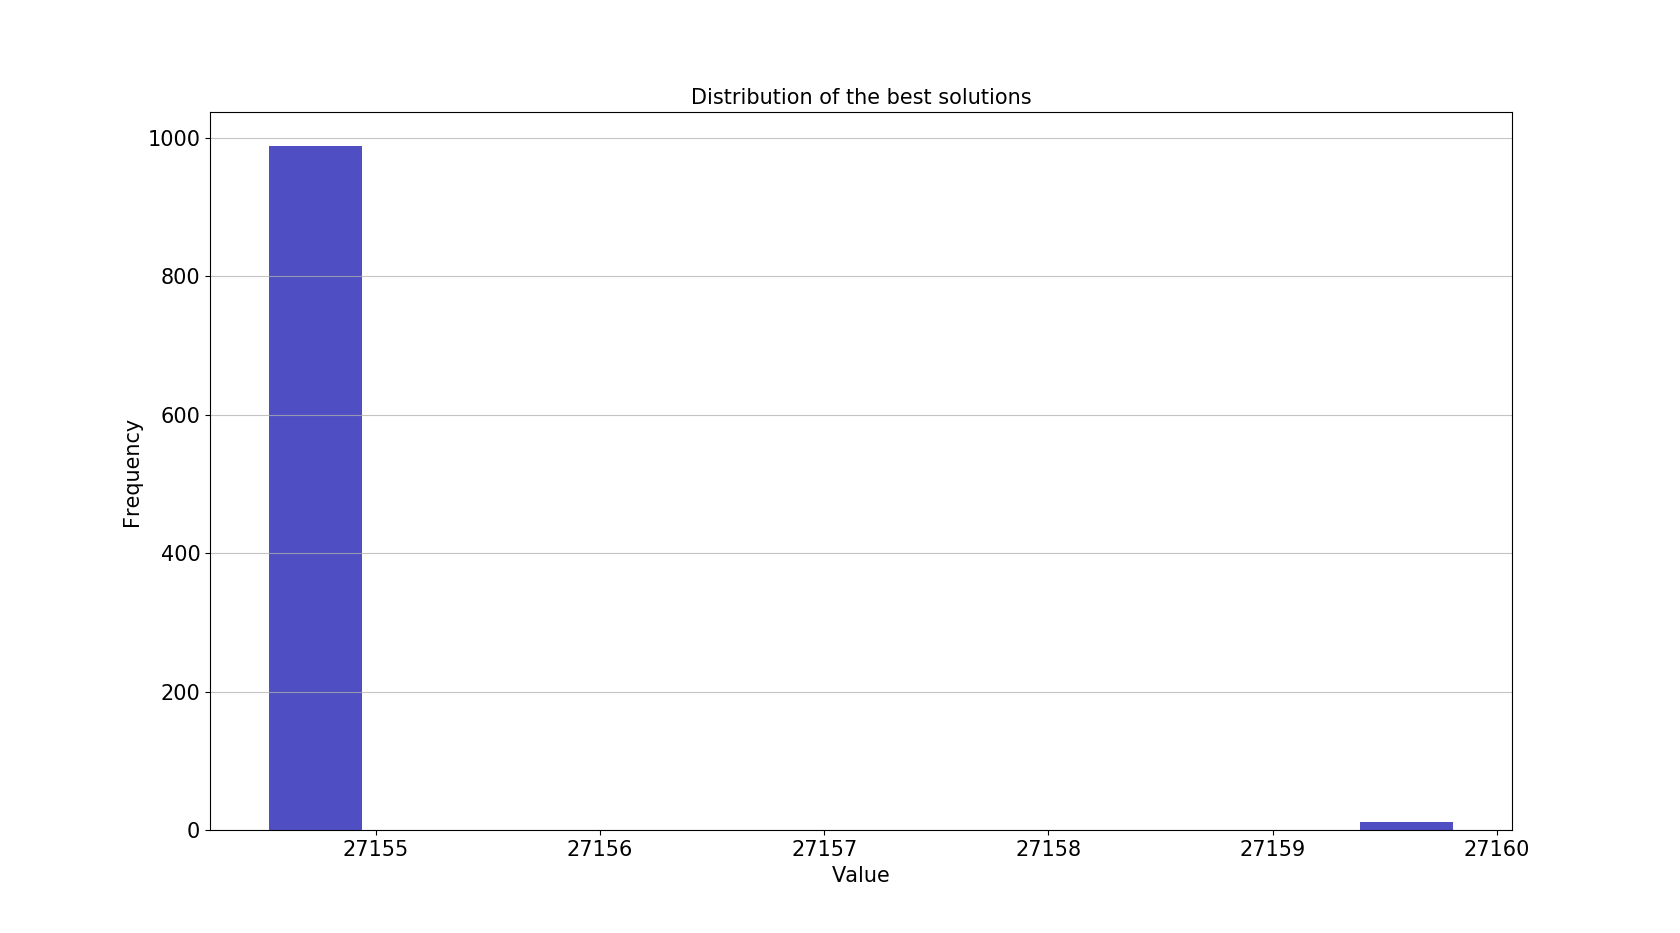
\includegraphics[width=1\textwidth]{hist_best.PNG}
%	\caption{Histogram of the best solutions attained during $ 1000 $ runs of the tour 29 problem.}
%	\centering
%\end{figure}


%\begin{figure}[h]
%	\label{fig:hist_mean_sol}
%	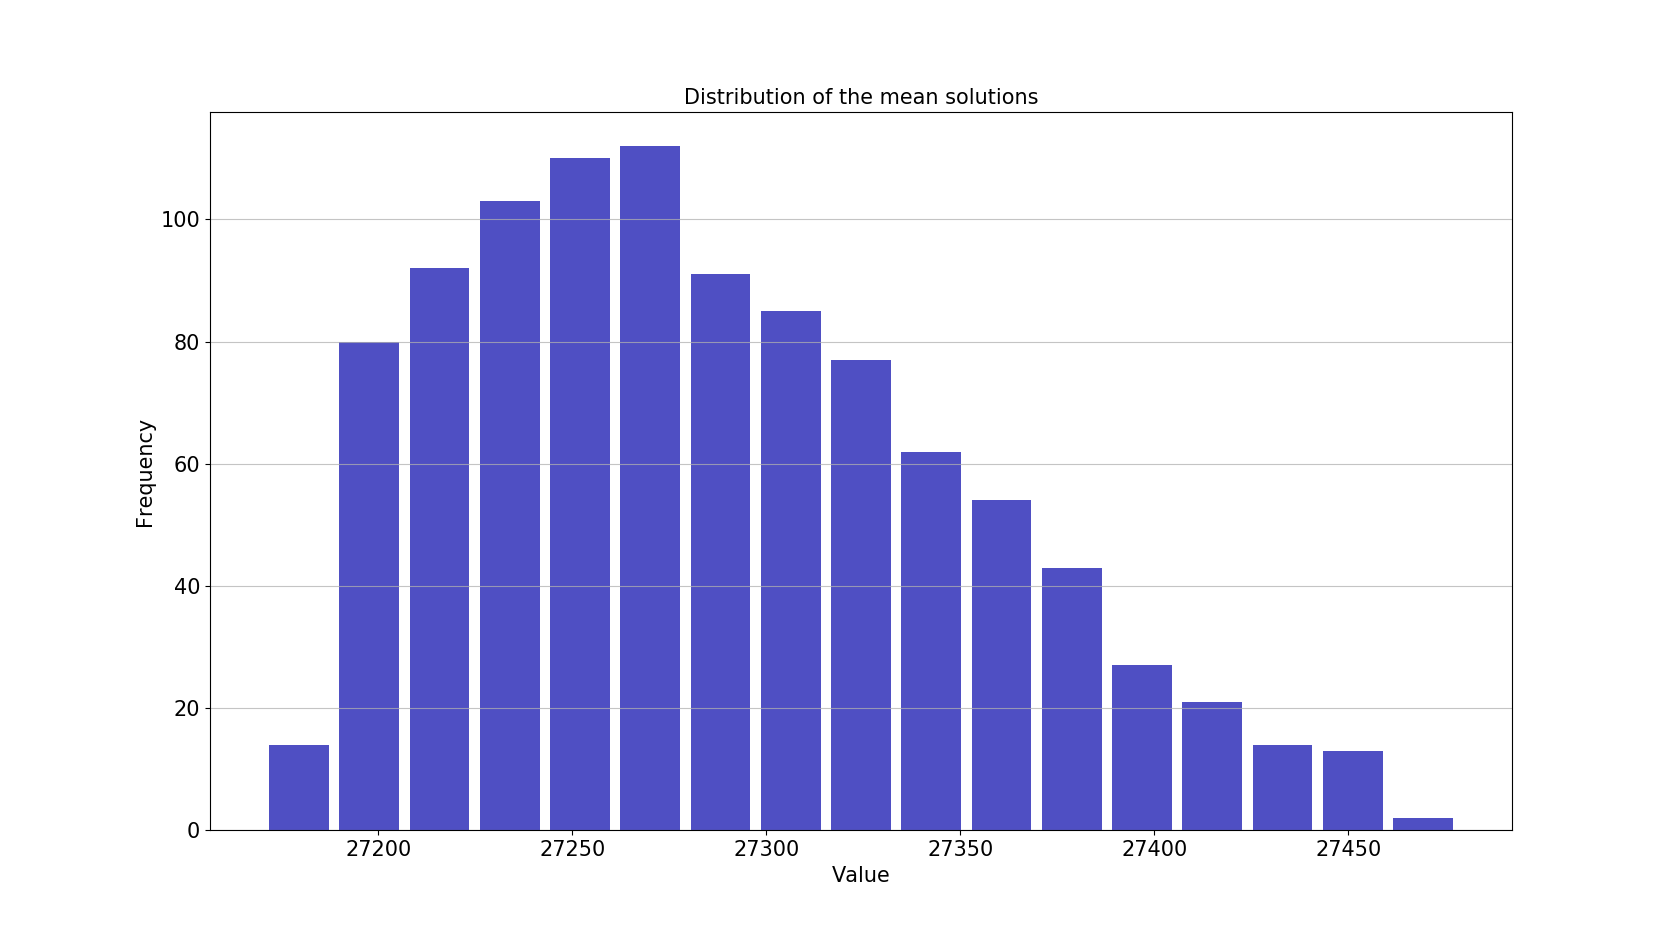
\includegraphics[width=1\textwidth]{hist_mean.PNG}
%	\caption{Histogram of the mean solutions attained during $ 1000 $ runs of the tour 29 problem.}
%	\centering
%\end{figure}




\subsection{tour100.csv}
The best tour length that is found has a cost of $ 7510.80 $.\footnote{The runtime warning encountered during testing is no problem. To remove it, redundant code is necessary that would make the implementation slower. }
The parameters used can be seen in Table \ref{t:parameters} and the convergence plot is given by Figure \ref{fig:convergence_tour100}.

\begin{figure}[h]
	
	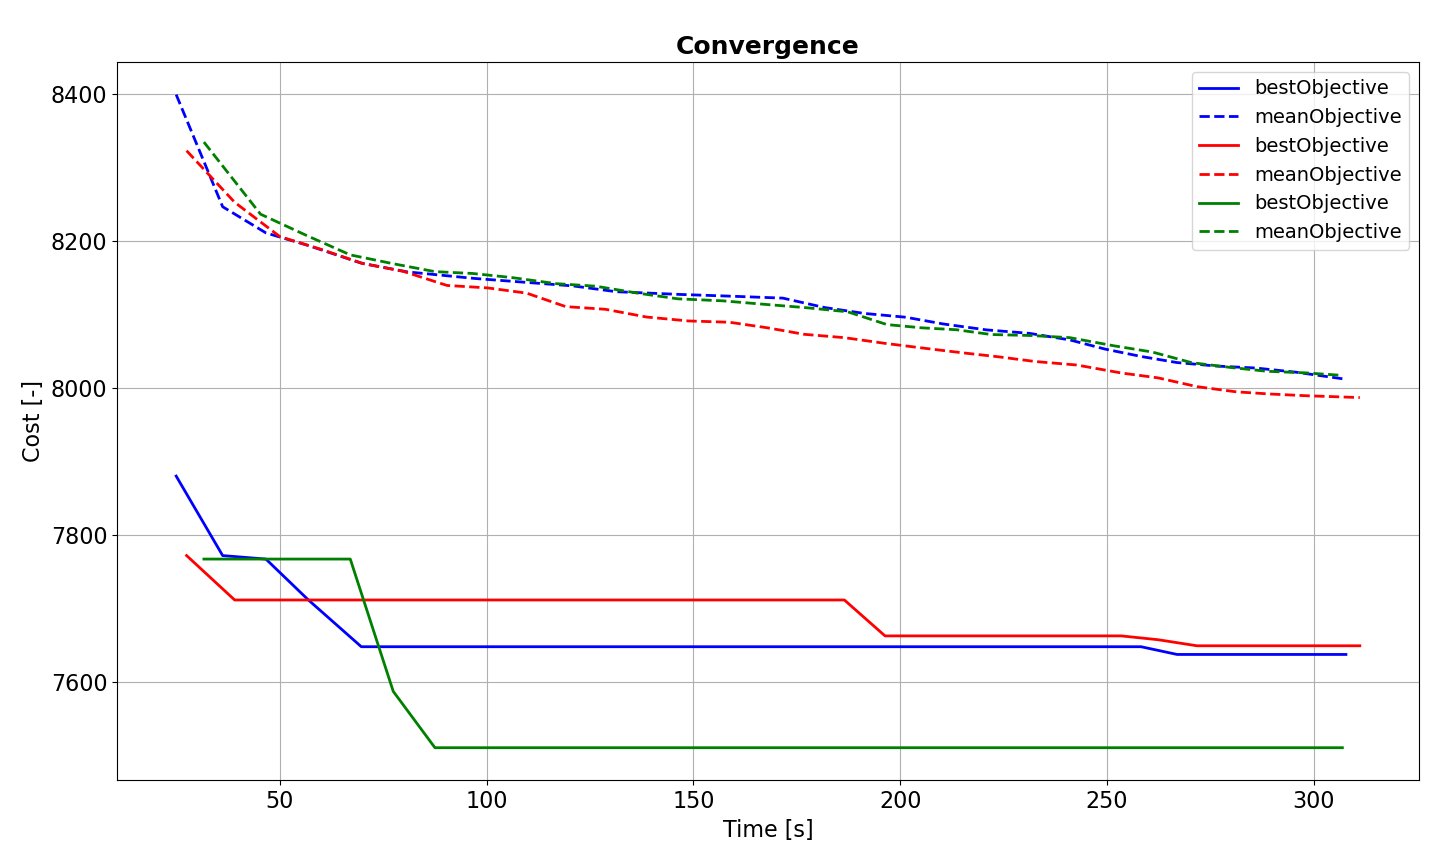
\includegraphics[width=1.0\textwidth]{convergence_tour100.PNG}
	\caption{Convergence plot of the tour 100 TSP}
	\label{fig:convergence_tour100}
	\centering
\end{figure}

Divergence stays sufficient high and reasonable solutions are attained. The best solution of the three has still an error of $ 2.1 \% $ with respect to the optimal solution. There is also more variability on the obtained solutions. It can be expected that when the algorithm is given more calculation resources, the variance will also decrease. All three solutions use the total $ 5 $ minutes of calculation time.

\subsection{tour194.csv}
The convergence plot can be seen in Figure \ref{fig:convergence_tour194}.
The best tour length that is found during these $ 3 $ runs has a cost of $9716.99  $ which means that all these three runs behaved worse than the mean best value identified during hyperparameters optimization. Here the mean best value was $ 9703.05 $ with a best objective value over $ 8 $ runs of $ 9569.90 $.
The parameters used can be seen in Table \ref{t:parameters}.

\begin{figure}[h]
	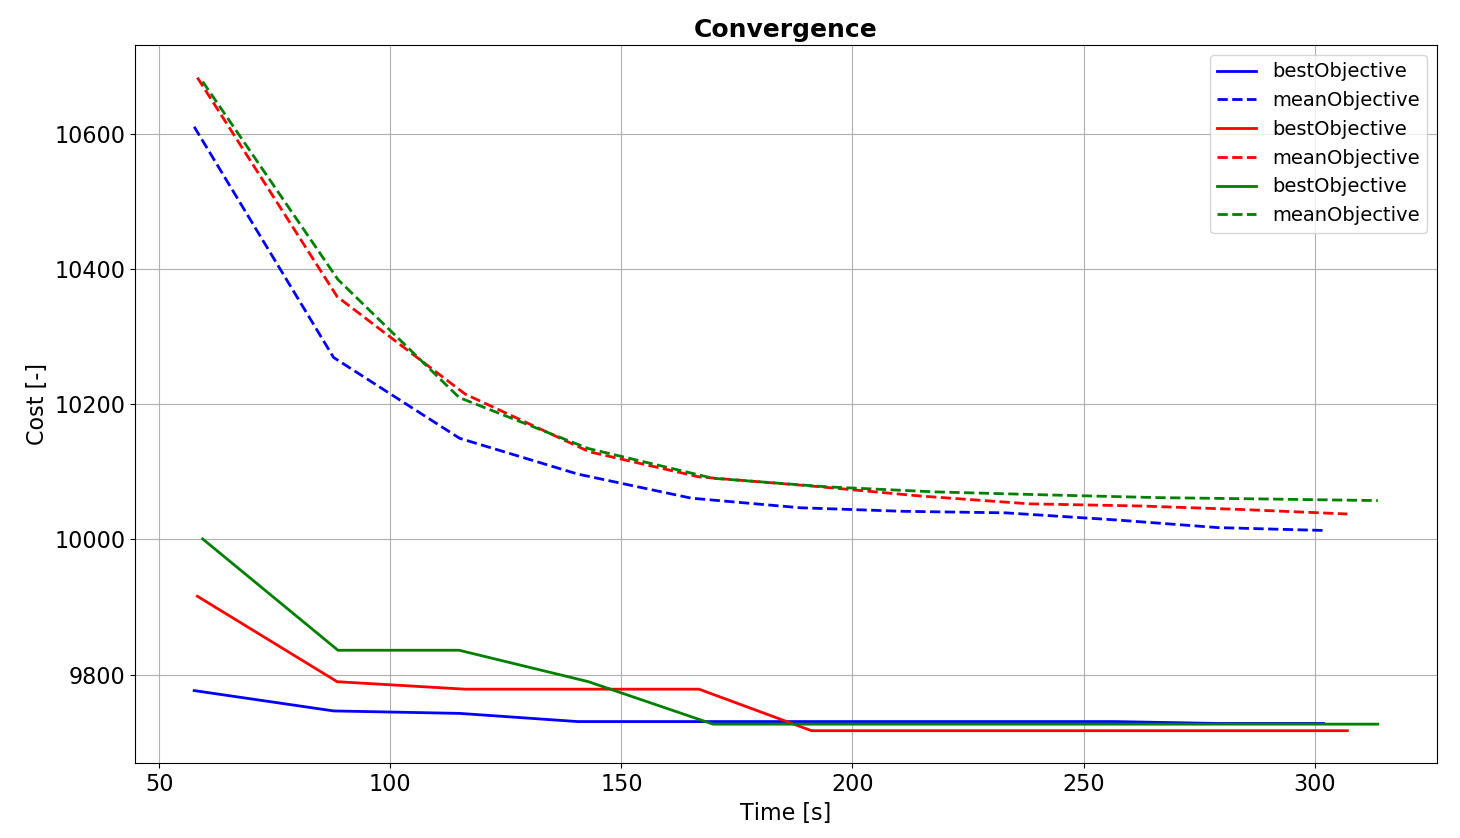
\includegraphics[width=1.0\textwidth]{convergence_tour194.PNG}
	\caption{Convergence plot of the tour 194 TSP}
	\label{fig:convergence_tour194}
	\centering
\end{figure}

Again it can be seen that divergence is not completely gone, because the mean objective value doesn't convergence towards the best objective value. There is some variability on the solutions that are found. The best objective value found has still an error of $ 6.0 \% $ with the optimal objective value of $ 9000 $


\subsection{tour929.csv}
The convergence plot can be seen in Figure \ref{fig:convergence_tour9292}.
The best tour length that is found  has a cost of $  103513.37 $.
The parameters used are picked by hand and are summarized by: 
\begin{itemize}
	\item Population size: $ 10 $
	\item Mutation rate: $ 0.02 $
	\item Amount of loops of the ``3-opt'' local search: $ 1 $
	\item Amount of times no different best solution: $ 100 $ 
\end{itemize}


\begin{figure}[h]
	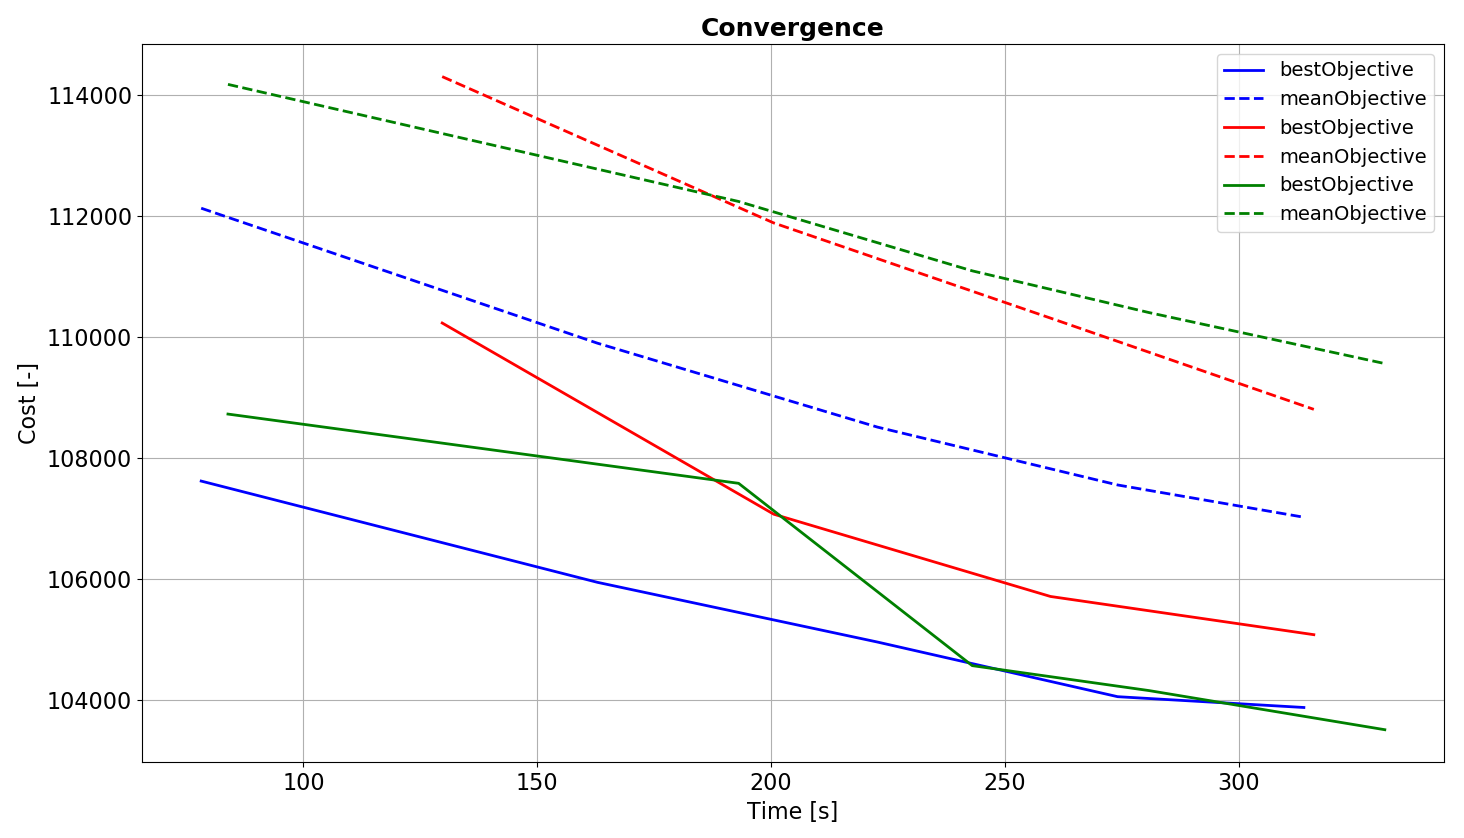
\includegraphics[width=1.0\textwidth]{convergence_tour9292.PNG}
	\caption{Convergence plot of the tour 929 TSP}
	\label{fig:convergence_tour9292}
	\centering
\end{figure}

It can be seen that only a small amount of iterations could be performed because of the high calculation load. Diversity is not instantaneous lost and the best objective value found, makes an error of $ 8.0 \% $ with the optimal objective value $ 95300 $.



\section{Critical reflection}

Evolutionary algorithms provide solution approaches that are very general and applicable to many problems. It can sometimes even be applied without in-depth knowledge of the problem. The ease of being general comes at the cost that it is often inferior to dedicated solution strategies that are often very time consuming to implement. Also, genetic algorithms are handy search methods for finding solutions for problems with a large solution domain e.g. parameters tuning for developed models.  


%\cite{fast_alg}
%\cite{inver_over}
\clearpage
\bibliographystyle{abbrv}
\bibliography{Evolutionary_Alg}

\end{document}
